\documentclass[fleqn,final]{beamer}
\mode<presentation>
{
  \usetheme{ForumStatBlau}
}
\usepackage{times}
\usepackage{etex}
\usepackage{amsmath,amssymb}
%\usepackage{sfmath} % for sans serif math fonts; wget http://dtrx.de/od/tex/sfmath.sty
\usepackage[english]{babel}
\usepackage[utf8]{inputenc}
\usepackage[ansinew]{inputenc}
\usepackage[orientation=portrait,size=a0,scale=1.25,debug]{beamerposter}
\usepackage{booktabs,array}
\usepackage{listings}
% \usepackage{picins}
\usepackage{graphicx}
\usepackage{xspace}
\usepackage{keyval}

\usepackage{wrapfig}
\usepackage{fp}
\usepackage{ifthen}
\usepackage[T1]{fontenc}
\usepackage{tikz,colortbl,pgf,pgfarrows,pgfnodes,pgfautomata,pgfheaps,pgfshade,eurosym, dsfont}

\usepackage{pgfplots}
%\pgfplotsset{compat=1.8}

\listfiles
\newcommand*{\signstream}{SignStream\texttrademark\xspace}
\newcommand{\WichtigFarbe}{\color{red}}%
\newcommand{\TextFarbe}{\color{black}}%



\def\bs{\boldsymbol}
\definecolor{darkblue}{rgb}{0.28,0,0.60}
\definecolor{hblue}{rgb}{0.70,0.7,1}
\definecolor{NR0}{rgb}{1,1,1}
\definecolor{NR1}{rgb}{1,1,0.8}
\definecolor{NR2}{rgb}{1,1,0.5}
\definecolor{NR3}{rgb}{1,1,0.25}
\definecolor{NR4}{rgb}{1,1,0.0}
\definecolor{NR5}{rgb}{1,0.75,0.0}
\definecolor{NR6}{rgb}{1,0.5,0.0}
\definecolor{NR7}{rgb}{1,0.25,0.0}
\definecolor{NR8}{rgb}{1,0,0.0}

\setbeamertemplate{navigation symbols}{}
\setbeamerfont{title}{series=\bfseries}

%\setbeamercolor{palette primary}{fg=yellow,bg=yellow} % changed this
%\setbeamercolor{palette secondary}{use=structure,fg=structure.fg!100!green} % changed this
%\setbeamercolor{palette tertiary}{use=structure,fg=structure.fg!100!green} % changed this
%\setbeamercolor{frametitle}{fg=UTblue}
\setbeamerfont{frametitle}{series=\bfseries}
\setbeamertemplate{frametitle}
{
\begin{centering}
\insertframetitle\vspace*{-4mm}\par
\end{centering}
}

\newcommand{\convD}{\stackrel{\text{d}}{\longrightarrow}}
\newcommand{\E}{\text{E}\,}
\newcommand{\var}{\text{V}\,}

% Display a grid to help align images
%\beamertemplategridbackground[1cm]
%\pgfdeclareimage[width=25cm]{CR}{graphs/CR}
\pgfdeclareimage[width=9.5cm]{RRMSE1}{RRMSE1}
\pgfdeclareimage[width=9.5cm]{RB1}{RB1}
\pgfdeclareimage[width=9.5cm]{RRMSEp1}{RRMSEp1}
\pgfdeclareimage[width=9.5cm]{RBp1}{RBp1}
\pgfdeclareimage[height=11cm]{histoposter1}{histoposter1}
\pgfdeclareimage[height=11cm]{histoposter2}{histoposter2}
\pgfdeclareimage[width=22cm]{Spatial}{Spatial}


\usepackage{float}
\usepackage{subfig}
%\usepackage[showframe]{geometry}
%\usepackage{enumitem}


\title{\huge Application of LDA topic model to song lyrics} %konkreter Titel!!
\author{\large Silvia Ventoruzzo}
\institute{Freie Universität Berlin} % (optional, but mostly needed)
\date{today}


\begin{document}

\begin{frame}
      
%%%%%%%%%%%%%%%%%%%%%%%%%%%%%%%%%%%%%%%%%%%%%%%%%%%%%%%%%%%%%%%%%%%%%%%%%%%%%%%%%
\vspace{-1cm} 
 \begin{columns}[t]
      \begin{column}{.50\linewidth}
        \begin{block}{\rule[-2.5mm]{0cm}{1cm}\textsc{1. Motivation}}


\begin{itemize}\small{
    \item Topic models are unsupervised learning methods to extract topics from a corpus of documents
    \item Latent Dirichlet Allocation (LDA) is "generative probabilistic model for collections of discrete data such as text corpora" [1]
    \item Commonly used methods to estimate the latent parameters: VEM [1] and Gibbs Sampling (Griffiths and Steyvers, 2004). VEM will be used in this project
    \item LDA can be used for general discrete data, but it is often used in the context of text mining
    \item We will try to obtain topics
}
\end{itemize}
\vspace{0.5cm}
%\textcolor{blue}{How do the proposed methods assist in improving the precision of small area prediction when the dependent variable is censored to particular intervals?	} 		%		}
\vspace{0.5cm}

\end{block}
\vspace{-1cm}
%%%%%%%%%%%%%%%%%%%%%%%%%%%%%%%%%%
%%%%%%%%%%%%%%%%%%%%%%%%%%%%%%%%%%%%%%%%%%%%%%%%%%%%%%%%%%%%%%%%%%%%%%%%%%%%%%%%%%%%%%%%%%%%%%%%%%%%%%%%%%%%%%%
%%%%%%%%%%%%%%%%%%%%%%%%%%%%%%%%%%%%%%%%%%%%%%%%%%%%%%%%%%%%%%%%%%%%%%%%%%%%%%%%%	 	

\begin{block}{\rule[-2.5mm]{0cm}{1cm}\textsc{2. Latent Dirichlet Allocation [1]}}
\begin{columns}[t]
\begin{column}{.47\linewidth}
{\small 
\vspace{-1.3cm}	
\begin{block}{\small{Model}}
\vspace{0.2cm}	
\begin{itemize}
    \item The corpus $D$ is a collection of $M$ documents: $D = \{d_1, ..., d_M\}$
    \item A document of the corpus $d_j$ is a sequence of $N_j$ words: $d_j = (w_1, ..., w_{N_j})$
    \item A word present in the corpus $w_i$ is an item from the vocabulary, that is the set of all words present in the corpus \citep{ponweiser2012latent}: $w_i \in \{1, ..., V\}$
\end{itemize}

\end{block}
}
\end{column}			

\begin{column}{.47\linewidth}
{\small 			
\vspace{-1.3cm}	
\begin{block}{\small{Generative process}}
\begin{itemize}
    \item For all topics $k \in \{1, ..., K\}$:
        \begin{enumerate}
            \item Choose a word distribution: $\beta_k \sim Dir(\delta)$
        \end{enumerate}
    \item For all documents $d_j$ where $j \in \{1, ..., M\}$:
        \begin{enumerate}
            \item Choose a topic distribution: $\theta_j \sim Dir(\alpha)$
            \item Assign topics for all words $w_i$ where $i \in \{1, ..., N_j\}$: $z_{j, i} \sim Mult(\theta_j)$
            \item Choose a word $w_i$: $w_{j, i} \sim Mult(\beta_{z_{j, i}})$
        \end{enumerate}
\end{itemize}

\end{block}
}
\end{column}
\end{columns}
\vspace{1cm}	
%%%%%%%%%%%%%%%%%%%%%%%%%%%%%%%%%%%%%%%%%%%%%%%%%%%%%%%%%%%%%%%%%%%%%%%%%%%%%%%%%
 	
%%%%%%%%%%%%%%%%%%%%%%%%%%%%%%%%%%%%%%%%%%%%%%%%%%%%%%%%%%%%%%%%%%%%%%%%%%%%%%%%%		



%%%%%%%%%%%%%%%%%%%%%%%%%%%%%%%%%%%%%
%%%%%%%%%%%%%%%%%%%%%%%%%%%%%%%%%%%%%%%%%%%%%%%%%%%%%%%%%%%%%%%%%%%%%%%%%%%%%%%%%%%%%%%%%%%%%%%%%%%%%%%%%%%%%%%%%%
%\vspace{0.2cm}
        
%%%%%%%%%%%%%%%%%%%%%%%%%%%%%%%%%%%%%%%%%%%%%%%%%%%%%%%%%%%%%%%%%%%%%%%%%%%%%%%%%

\begin{columns}[t]
\begin{column}{.47\linewidth}
{\small 
\vspace{-1.3cm}	
\begin{block}{\small{Estimation}}
\vspace{0.2cm}	
Optimize log-likelihood of the marginal distribution of the documents $d_j$ with respect to the coefficients $\alpha$ and $\beta$:
\small{
\begin{align*}
    \resizebox{0.95\hsize}{!}{$p(d_j|\alpha, \beta) = \int p(\theta|\alpha) \bigg(\prod_{i=1}^{N_j}\sum_{z_{j,i}} p(z_{j,i}|\theta)p(w_{j,i}|z_{j,i}, \beta)\bigg) \,d\theta$}
\end{align*}
}

\end{block}
}
\end{column}			

\begin{column}{.47\linewidth}
{\small 			
\vspace{-1.3cm}	
\begin{block}{\small{Inference}}
Since the function $p(d_j|\alpha, \beta)$ is intractable, variational Bayesian inference is used with the variational parameters $\gamma$ and $\phi$:
\small{
\begin{align*}
    (\gamma^*, \phi^*) = \argmin_{(\gamma, \phi)} D_{KL}(q(\theta, \textbf{z}|\gamma, \phi)||p(\theta, \textbf{z}|\textbf{d}, \alpha, \beta))
\end{align*}
}

\end{block}
}
\end{column}

\end{columns}

%\vspace{-0.7cm}	
{\small
{\color{blue}{Variational expectation-maximization (VEM):}}
\begin{itemize}
    \item \textbf{E-step}: Find $\{\gamma^*_j, \phi^*_j\}$, where $d_j \in D$, i.e. the optimal values of the variational parameters $\gamma$ and $\phi$ for each document
    \item \textbf{M-step}: Maximize the resulting lower bound on the log-likelihood with respect to the latent parameters $\alpha$ and $\beta$
\end{itemize}
}

%%%%%%%%%%%%%%%%%%%%%%%%%%%%%%%%%%%%%%%%%%%%%%%%%%%%%%%%%%%%%%%%%%%%%%%%%%%%%%%%%%%%%%%%%%%%%%%%%%%%%%%%%%%%%%%%%%
\vspace{1cm}
        
%%%%%%%%%%%%%%%%%%%%%%%%%%%%%%%%%%%%%%%%%%%%%%%%%%%%%%%%%%%%%%%%%%%%%%%%%%%%%%%%%

\begin{columns}[t]
\begin{column}{.47\linewidth}
{\small 
\vspace{-1.3cm}	
\begin{block}{\small{Number of topics}}
\vspace{0.2cm}	
{\color{blue}{Methods to derive the appropriate number of topics:}}
\begin{itemize}
    \item Perplexity of hold-out set [1]
    \item Metric based on the average cosine distance among semantic clusters [2]
    \item Metric based on the information divergence between pairs of topics [3]
    \item Metric based on the divergence among stochastic matrices [4]
    \item Human judgment [5]
\end{itemize}

\end{block}
}
\end{column}			

\begin{column}{.47\linewidth}
{\small 			
\vspace{-1.3cm}	
\begin{block}{\small{Interpretation}}


\end{block}
}
\end{column}

\end{columns}

\end{block}	

%%%%%%%%%%%%%%%%%%%%%%%%%%%%%%%%%%%%%%%%%%%%%%%%%%%%%%%%%%%%%%%%%%%%%%%%%

%\begin{block}{\rule[-2.5mm]{0cm}{1cm}\textsc{3. R packages}}
%{\color{blue}{The following R packages were employed:}}
%\begin{itemize}
%    \item \texttt{topicmodels}: For LDA model and perplexity
%    \item \texttt{ldatuning}: For other metrics
%    \item \texttt{quanteda}: For data preparation
%    \item \texttt{stopwords}: For the vector of stopwords
%    \item \texttt{tidytext}: For the extraction of the LDA parameters
%\end{itemize}
%\end{block}

\begin{block}{\rule[-2.5mm]{0cm}{1cm}\textsc{3. Dataset}}

200 songs from 17 artists and 5 music genres between 2010 and 2016.

\begin{figure}[ht]
\centering
\subfloat{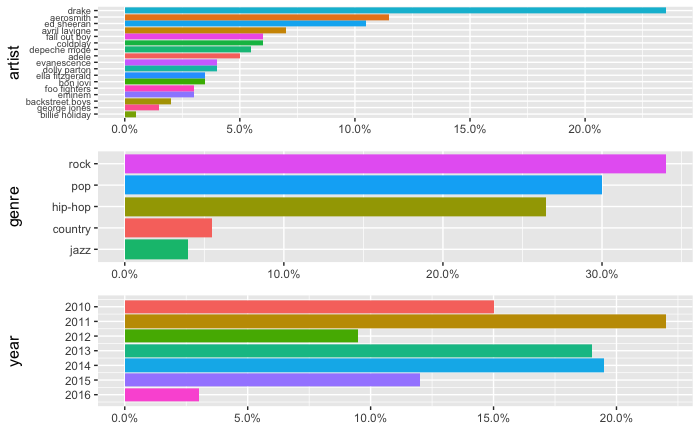
\includegraphics[width=0.5\textwidth]{varplots.png}}
\subfloat{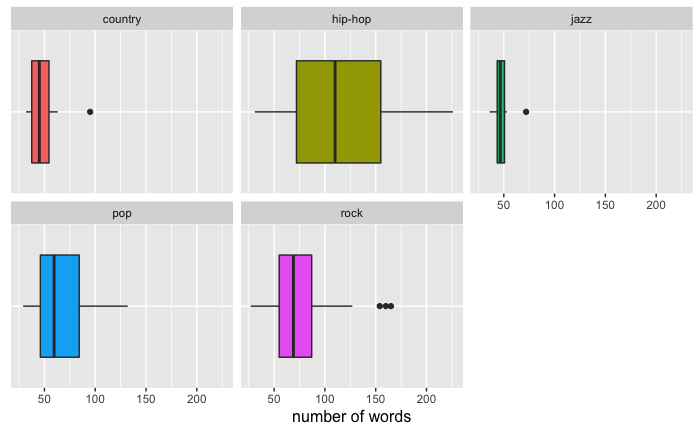
\includegraphics[width=0.5\textwidth]{wordsgenres.png}}
%\caption{Sentiments according to the different lexicons with respect to genre and artist}
\end{figure}
\begin{figure}[ht]
\centering
\subfloat{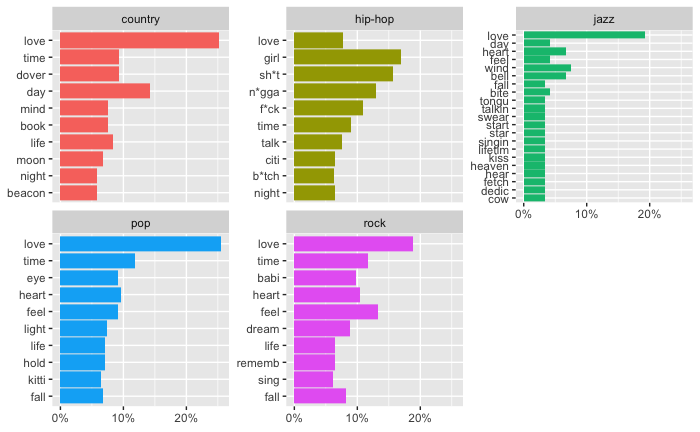
\includegraphics[width=0.5\textwidth]{genre_words.png}}
\subfloat{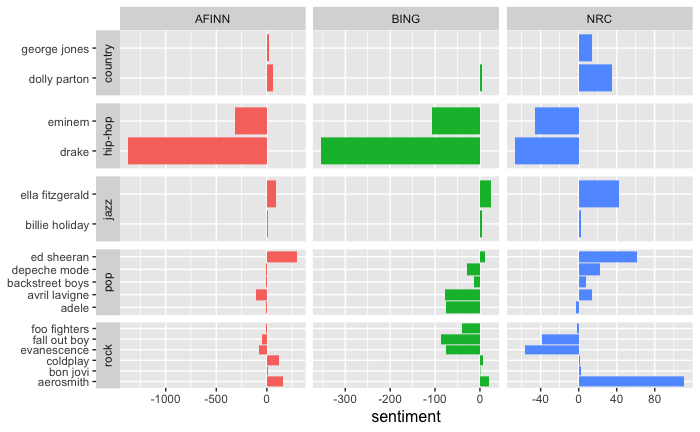
\includegraphics[width=0.5\textwidth]{sentiments_artist.png}}
%\caption{Sentiments according to the different lexicons with respect to genre and artist}
\end{figure}

\vspace{-0.5cm}                                            

\end{block}


%%%%%%%%%%%%%%%%%%%%%%%%%%%%%%%%%%%%%%%%%%%%%%%%%%%%%%%%%%%%%%%%%%%%%%%%%%%%%%%%%%%%%%%%%%%%%%%%%%%%%%%%%%%%%%%%%%%%%%%%%%%%%%%%



  \end{column}
%%%%%%%%%%%%%%%%%%%%%%%%%%%%%%%%%%%%%%%%%%%%%%%%%%%%%%%%%%%%%%%%%%%%%%%%%%%%%%%%%
%%%%%%%%%%%%%%%%%%%%%%%%%%%%%%%%%%%%%%%%%%%%%%%%%%%%%%%%%%%%%%%%%%%%%%%%%%%%%%%%%
%%%%%%%%%%%%%%%%%%%%%%%%%%%%%%%%%%%%%%%%%%%%%%%%%%%%%%%%%%%%%%%%%%%%%%%%%%%%%%%%%
%%%%%%%%%%%%%%%%%%%%%%%%%%%%%%%%%%%%%%%%%%%%%%%%%%%%%%%%%%%%%%%%%%%%%%%%%%%%%%%%%
%%%%%%%%%%%%%%%%%%%%%%%%%%%%%%%%%%%%%%%%%%%%%%%%%%%%%%%%%%%%%%%%%%%%%%%%%%%%%%%%%

    \begin{column}{.46\linewidth}
  
  %%%%%%%%%%%%%%%%%%%%%%%%%%%%%%%%%%%%%%%%%%%%%%%%%%%%%%%%%%%%%%%%%%%%%%%%%%%%%%%%%%%%%%%%%%%%%%%%%%%%%%%%%%%%%%%%%%%%%%%%%%%%%%%%%%%%%%%%%%

    
%%%%%%%%%%%%%%%%%%%%%%%%%%%%%%%%%%%%%%%%%%%%%%%%%%%%%%%%%%%%%%%%%%%%%%%%%
\begin{block}{\rule[-2.5mm]{0cm}{1cm}\textsc{4. Implementation}}

\vspace{-1.3cm}
\begin{column}{.98\linewidth}
\begin{block}{\small{Number of topics}}

\begin{figure}[ht]
\centering
\subfloat{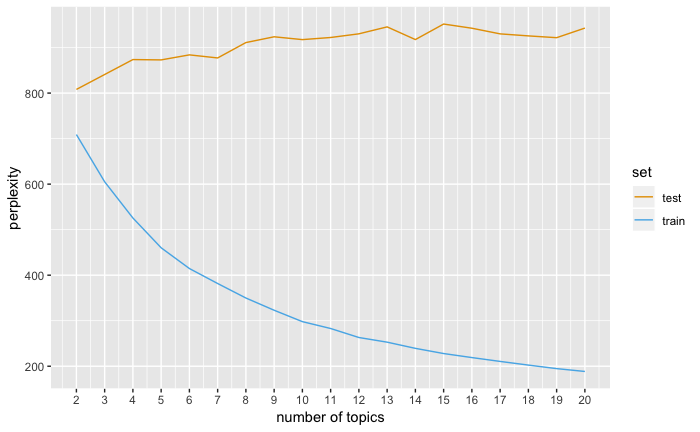
\includegraphics[width=0.5\textwidth]{ntopicperp.png}}
\subfloat{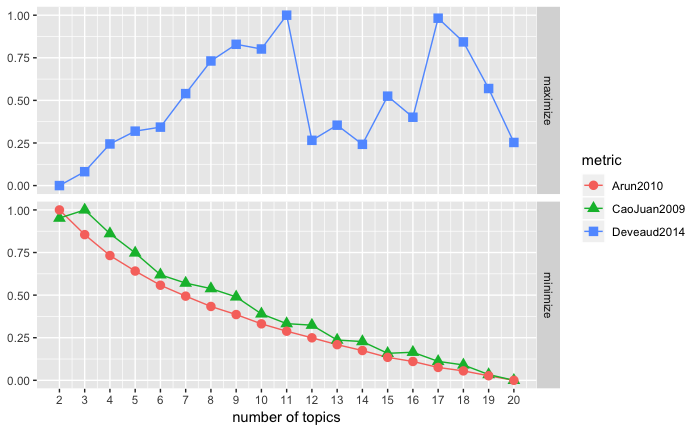
\includegraphics[width=0.5\textwidth]{ntopics.png}}
%\caption{Scaled distribution of metrics' values with respect to the number of topics}
\centering
\label{figure:ntopics}
\end{figure}

\end{block}
\end{column}
\vspace{-1.3cm}

\begin{columns}[t]
\begin{column}{.47\linewidth}
{\small 
\vspace{-1.3cm}	
\begin{block}{\small{Per-topic-per-word probability}}
\vspace{0.2cm}	
\begin{figure}[H]
	\centering
		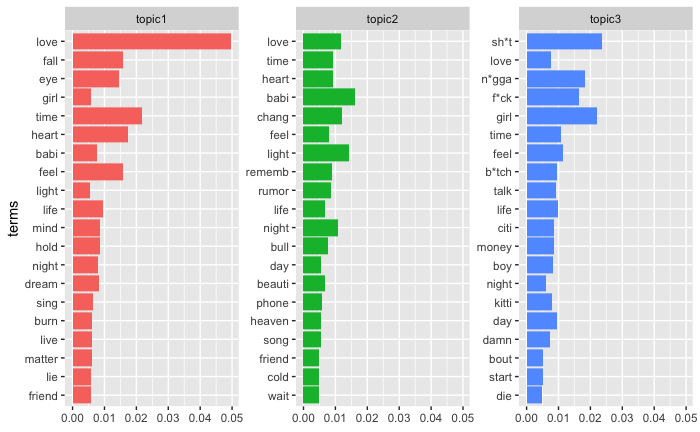
\includegraphics[width=\textwidth]{topic_word_3_20.png}
%	\label{figure:textlength}
\end{figure}

\end{block}
}
\end{column}			

\begin{column}{.47\linewidth}
{\small 			
\vspace{-1.3cm}	
\begin{block}{\small{Per-genre-per-topic probability}}
\begin{figure}[H]
	\centering
		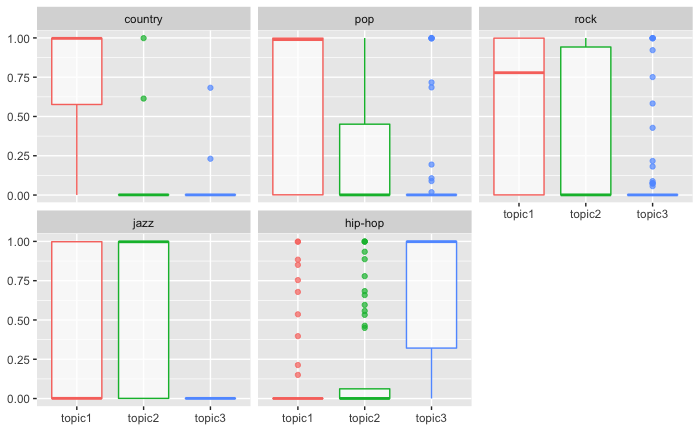
\includegraphics[width=\textwidth]{genre_topic_3.png}
%	\label{figure:textlength}
\end{figure}

\end{block}
}
\end{column}
\end{columns}


\begin{column}{.98\linewidth}
\begin{block}{\small{Per-artist-per-topic probability}}
\begin{figure}[H]
\centering
%\begin{columns}
%\begin{column}
\subfloat{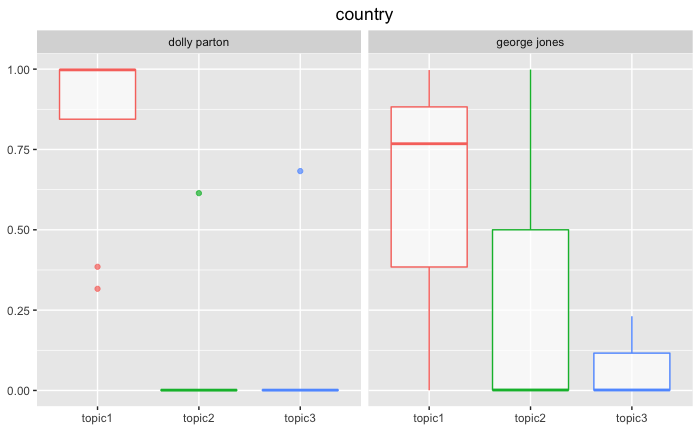
\includegraphics[width=0.3\textwidth]{country_topic.png}}
\subfloat{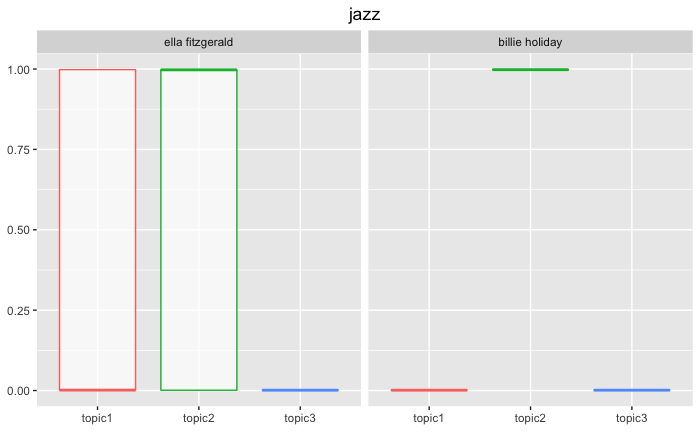
\includegraphics[width=0.3\textwidth]{jazz_topic.png}}
\subfloat{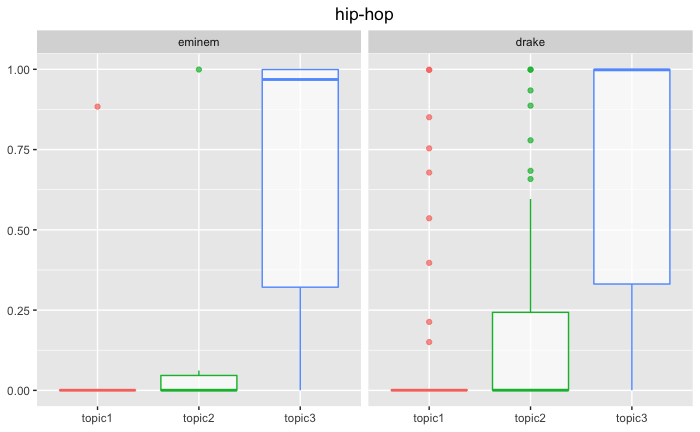
\includegraphics[width=0.3\textwidth]{hiphop_topic.png}}
\end{figure}
%\end{column}
%\begin{column}
\begin{figure}[H]
\centering
\subfloat{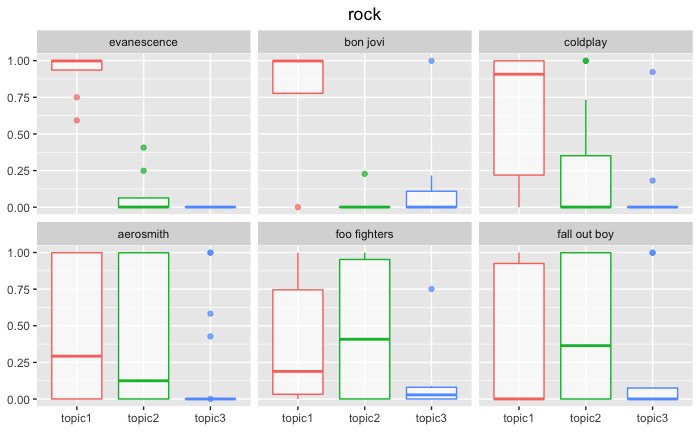
\includegraphics[width=0.45\textwidth]{rock_topic.png}}
\subfloat{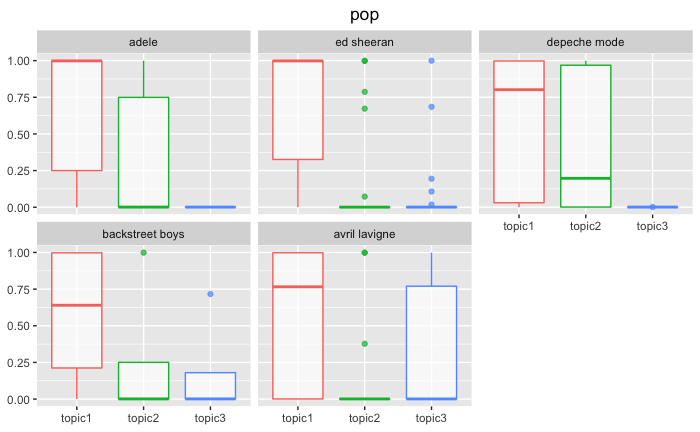
\includegraphics[width=0.45\textwidth]{pop_topic.png}}
%\end{column}
%\end{columns}
%\label{figure:artist_topic}
\end{figure}


		
\end{block}
\end{column}
\end{block}	 	
\vspace{-1cm}






%%%%%%%%%%%%%%%%%%%%%%%%%%%%%%%%%%%%%%%%%%%%%%%%%%%%%%%%%%%%%%%%%%%%%%%%%%%%%%%%%%%%%%%%%%%%%%%%%%%%%%%%%%%%%%%%%%%%%%%%%%%%%%%%%%%%%%%%%%

	 	
\begin{block}{\rule[-2.5mm]{0cm}{1cm}\textsc{5. Results and conclusions}}

\begin{itemize}
\item \textcolor{blue}{According to LDA with VEM estimation, the dataset can be split into 3 topics:}
    \begin{enumerate}
        \item \textcolor{blue}{Romantic love}: mostly Pop and Country songs, part of Rock ones
        \item \textcolor{blue}{Everyday life}: primarily Jazz songs, part of Rock ones 
        \item \textcolor{blue}{Race fight}: mainly Hip-Hop songs [FIND BETTER WORD]
    \end{enumerate}
\item There is, in general, no clear separation of topics inside genres and artists
\item Increasing the number of topics improves the definition of topics for artists, but reduces the interpretability

%\item \textbf{Further research:} How can possible violations of model assumptions be detected? How can transformations be applied for handling non-normally distributed error terms?  
\end{itemize}





		\end{block}	 	
%%%%%%%%%%%%%%%%%%%%%%%%%%%%%%%%%%%%%%%%%%%%%%%%%%%%%%%%%%%%%%%%%%%%%%%%%%%%%%%%%		
			
 \end{column}
\end{columns}



\vspace{-1cm}
   \begin{block}{References}
   \vspace{-0.3cm}

{\footnotesize

\noindent [1]  Blei, D. M., Ng, A. Y., \& Jordan, M. I. (2003). Latent dirichlet allocation. Journal of machine Learning research, 3 (Jan), 993–1022\\

\noindent [2] Cao, J., Xia, T., Li, J., Zhang, Y., \& Tang, S. (2009). A density-based method for adaptive lda model selection. Neurocomputing, 72 (7-9), 1775–1781.\\

\noindent [3] Arun, R., Suresh, V., Madhavan, C. V., \& Murthy, M. N. (2010). On finding the natural number of topics with latent dirichlet allocation: Some observations. In Pacific-asia conference on knowledge discovery and data mining (pp. 391–402)\\

\noindent [4] Deveaud, R., SanJuan, E., \& Bellot, P. (2014). Accurate and effective latent concept modeling for ad hoc information retrieval. Document numérique, 17 (1), 61–84.\\

\noindent [5] Chang, J., Gerrish, S., Wang, C., Boyd-Graber, J. L., \& Blei, D. M. (2009). Reading tea leaves: How humans interpret topic models. In Advances in neural information processing systems (pp. 288–296).\\

%\noindent [6] Dempster, A., Laird, N., \& Rubin, D. (1977),
%Maximum likelihood from incomplete data via the em algorithm. 
%Journal of the Royal Statistical Society. Series B (Methodological),
%39(1):1 - 38.\\

%\noindent [7] Groß, M., Rendtel, U., Schmid, T., Schmon, S.\& Tzavidis, N. (2016),
%Estimating the density of ethnic minorities and aged people in Berlin: multivariate kernel density estimation applied to sensitive georeferenced administrative data protected via measurement error.
%Journal of the Royal Statistical Society. Series A.
%\\


}


\end{block}

\end{frame}


\end{document}

